\documentclass[11pt,a4paper]{article}

\usepackage{ifxetex}
\RequireXeTeX

\usepackage[a4paper,tmargin=1in,bmargin=1.3in,lmargin=1in,rmargin=1in]{geometry}

% bookmarks in PDF
\usepackage[colorlinks=true,linkcolor=blue,urlcolor=blue,bookmarksopen=true]{hyperref}
\usepackage[depth=3]{bookmark}
% open file with zoom to page width
\hypersetup{pdfstartview={FitH top}}

% math package
\usepackage{amsmath}

% customizing fonts
\usepackage{fontspec}
\usepackage{xcolor}
\usepackage{titlesec}
\setsansfont{Fira Sans}
\setmonofont{JetBrains Mono NL}[Scale=0.8]
\setmainfont{Dijakritika}
\titleformat*{\section}{\Large\bfseries\sffamily}
\titleformat*{\subsection}{\bfseries\sffamily}

% image handling
\usepackage{graphicx}
\usepackage{forest}
\usepackage{tikz}
\usetikzlibrary{arrows,petri,topaths,arrows.meta,automata,calc,shapes.multipart,chains,shapes.gates.logic.US,matrix}
\usepackage{tkz-berge}
\usepackage[position=top]{subfig}
\tikzstyle{branch}=[fill,shape=circle,minimum size=3pt,inner sep=0pt]

% syntax highligting
\usepackage{minted}

% custom headers and footers
\usepackage{fancyhdr}
\pagestyle{fancy}
\fancyhf{}
\chead{ASP primeri}
\cfoot{Page \thepage}
\setlength{\headheight}{46pt}

\begin{document}

\section{Nizovi}

\subsection{Problem holandske zastave}

The quicksort algorithm for sorting arrays proceeds recursively -- it selects
an element (the ``pivot''), reorders the array to make all the elements less
than or equal to the pivot appear first, followed by all the elements greater
than the pivot. The two subarrays are then sorted recursively.

Implemented naively, quicksort has large run times and deep function call
stacks on arrays with many duplicates because the subarrays may differ
greatly in size. One solution is to reorder the array so that all elements
less than the pivot appear first, followed by elements equal to the pivot,
followed by elements greater than the pivot. This is known as Dutch national
flag partitioning, because the Dutch national flag consists of three
horizontal bands, each in a different color.

As an example, assuming that blue precedes white and white precedes red,
Figure \ref{fig:dutchflag} is a valid partitioning for Figure
\ref{fig:flagbefore}. If red precedes blue and blue precedes white, Figure
\ref{fig:russianflag} is a valid partitioning for Figure \ref{fig:flagbefore}.

Generalizing, suppose $A = (0,1,2,0,2,1,1)$, and the pivot index is 3. Then 
$A[3] = 0$, so (0,0,1,2,2,1,1) is a valid partitioning. For the same array,
if the pivot index is 2, then $A[2] = 2$, so the arrays (0,1,0,1,1,2,2) as 
well as (0,0,1,1,1,2,2) are valid partitionings.

\begin{figure}[h]
  \centering
  \subfloat[Before partitioning\label{fig:flagbefore}]{
    \begin{tikzpicture}[scale=0.3]
      \draw [fill=blue] (0,0) rectangle (16,1) {};
      \draw [fill=red] (0,1) rectangle (16,2) {};
      \draw [fill=blue] (0,2) rectangle (16,3) {};
      \draw [fill=blue] (0,3) rectangle (16,4) {};
      \draw [fill=white] (0,4) rectangle (16,5) {};
      \draw [fill=white] (0,5) rectangle (16,6) {};
      \draw [fill=red] (0,6) rectangle (16,7) {};
      \draw [fill=red] (0,7) rectangle (16,8) {};
      \draw [fill=white] (0,8) rectangle (16,9) {};
    \end{tikzpicture}
  }
  \hfil
  \subfloat[Three-way partitioning resembling the Dutch national flag\label{fig:dutchflag}]{
    \begin{tikzpicture}[scale=0.3]
      \draw [fill=blue] (0,0) rectangle (16,1) {};
      \draw [fill=blue] (0,1) rectangle (16,2) {};
      \draw [fill=blue] (0,2) rectangle (16,3) {};
      \draw [fill=white] (0,3) rectangle (16,4) {};
      \draw [fill=white] (0,4) rectangle (16,5) {};
      \draw [fill=white] (0,5) rectangle (16,6) {};
      \draw [fill=red] (0,6) rectangle (16,7) {};
      \draw [fill=red] (0,7) rectangle (16,8) {};
      \draw [fill=red] (0,8) rectangle (16,9) {};
    \end{tikzpicture}
  }
  \hfil
  \subfloat[Another three-way partitioning: the Russian national flag\label{fig:russianflag}]{
    \begin{tikzpicture}[scale=0.3]
      \draw [fill=red] (0,0) rectangle (16,1) {};
      \draw [fill=red] (0,1) rectangle (16,2) {};
      \draw [fill=red] (0,2) rectangle (16,3) {};
      \draw [fill=blue] (0,3) rectangle (16,4) {};
      \draw [fill=blue] (0,4) rectangle (16,5) {};
      \draw [fill=blue] (0,5) rectangle (16,6) {};
      \draw [fill=white] (0,6) rectangle (16,7) {};
      \draw [fill=white] (0,7) rectangle (16,8) {};
      \draw [fill=white] (0,8) rectangle (16,9) {};
    \end{tikzpicture}
  }
\end{figure}

\textbf{Challenge:} Write a program that takes an array $A$ and an index $i$
into $A$, and rearranges the elements such that all elements less than $A[i]$
(the ``pivot'') appear first, followed by elements equal to the pivot,
followed by elements greater than the pivot.

\textbf{Hint:} Think about the partition step in quicksort.

\textbf{Solution:} The problem is trivial to solve with $O(n)$ additional
space, where $n$ is the length of $A$. We form three lists, namely, elements
less than the pivot, elements equal to the pivot, and elements greater than
the pivot. Consequently, we write these values into $A$. The time complexity
is $O(n)$.

We can avoid using $O(n)$ additional space at the cost of increased time
complexity as follows. In the first stage, we iterate through $A$ starting
from index 0, then index 1, etc. In each iteration, we seek an element smaller
than the pivot -- as soon as we find it, we move it to the subarray of smaller
elements via an exchange. This moves all the elements less than the pivot to
the start of the array. The second stage is similar to the first one, the
difference being that we move elements greater than the pivot to the end of
the array. Code illustrating this approach is shown below.

\begin{minted}[frame=lines]{python}
RED, WHITE, BLUE = range(3)

def dutch_flag_partition(pivot_index, A):
    pivot = A[pivot_index]
    # First pass: group elements smaller than pivot.
    for i in range(len(A)):
        # Look fot a smaller element.
        for j in range(i + 1, len(A)):
            if A[j] < pivot:
                A[i], A[j] = A[j], A[i]
                break
    # Second pass: group elements larger than pivot.
    for i in reversed(range(len(A))):
        if A[i] < pivot: 
            break
        # Look for a larger element. Stop when we reach an element less than 
        # pivot, since first pass has moved them to the start of A.
        for j in reversed(range(i)):
            if A[j] > pivot:
                A[i], A[j] = A[j], A[i]
                break
\end{minted}

The additional space complexity is now $O(1)$, but the time complexity is
$O(n^2)$, e.g., if $i = n/2$ and all elements before $i$ are greater than
$A[i]$, and all elements after $i$ are less than $A[i]$. Intuitively, this
approach has bad time complexity because in the first pass when searching for
each additional element smaller than the pivot we start from the beginning,
However, there is no reason to start from so far back -- we can begin from the
last location we advanced to. (Similar comments hold for the second pass.)

To improve time complexity, we make a single pass and move all the elements
less than the pivot to the beginning. In the second pass we move the larger
elements to the end. It is easy to perform each pass in a single iteration,
moving out-of-place elements as soon as they are discovered.

\begin{minted}[frame=lines]{python}
RED, WHITE, BLUE = range(3)

def dutch_flag_partition(pivot_index, A):
    pivot = A[pivot_index]
    # First pass: group elements smaller than pivot
    smaller = 0
    for i in range(len(A)):
        if A[i] < pivot:
            A[i], A[smaller] = A[smaller], A[i] 
            smaller += 1
    # Second pass: group elements larger than pivot.
    larger = len(A) - 1
    for i in reversed(range(len(A))):
        if A[i] < pivot: 
            break
        elif A[i] > pivot:
            A[i], A[larger] = A[larger] , A[i]
            larger -= 1
\end{minted}

The algorithm we now present is similar to the one sketched above. The main
difference is that it performs classification into elements less than, equal
to, and greater than the pivot in a single pass. This reduces runtime, at the
cost of a trickier implementation. We do this by maintaining four subarrays:
\emph{bottom} (elements less than pivot), \emph{middle} (elements equal to
pivot), \emph{unclassified}, and \emph{top} (elements greater than pivot).
Initially, all elements are in \emph{unclassified}. We iterate through
elements in \emph{unclassified}, and move elements into one of \emph{bottom},
\emph{middle}, and \emph{top} groups according to the relative order between
the incoming unclassified element and the pivot.

As a concrete example, suppose the array is currently $A =
(-3,0,-1,1,1,?,?,?,4,2)$, where the pivot is 1 and ? denotes unclassified
elements. There are three possibilities for the first unclassified element,
$A[5]$.
\begin{itemize}
  \item $A[5]$ is less than the pivot, e.g., $A[5] = -5$. We exchange it with
    the first 1, i.e., the new array is $(-3, 0, -1, -5, 1, 1, ?, ?, 4, 2)$. 
  \item $A[5]$ is equal to the pivot, i.e., $A[5] = 1$. We do not need to move
    it, we just advance to the next unclassified element, i.e., the array is
    $(-3,0,-1,1,1,1,?,?,4,2)$. 
  \item $A[5]$ is greater than the pivot, e.g., $A[5] = 3$. We exchange it 
    with the last unclassified element, i.e., the new array is 
    $(-3,0,-1,1,1,?,?,3,4,2)$. 
\end{itemize}
    
Note how the number of unclassified elements reduces by one in each case.

\begin{minted}[frame=lines]{python}
RED, WHITE, BLUE = range(3)

def dutch_flag_partition(pivot_index, A):
    pivot = A[pivot_index]
    # Keep the following invariants during partitioning:
    # botton group: A[:smaller]
    # middle gtoup: A[smaller:equal]
    # unclassified group: A[equal:larger]
    # top group: A[larger]
    smaller, equal, larger = 0, 0, len(A)
    # Keep iterating as long as there is an unclassified elenent
    while equal < larger:
        # A[equal] is the incoming unclassified element
        if A[equal] < pivot:
            A[smaller], A[equal] = A[equal], A[smaller]
            smaller, equal = smaller + 1, equal + 1 
        elif A[equal] == pivot:
            equal += 1
        else:  # A[equal] > pivot.
            larger -= 1
            A[equal], A[larger] = A[larger], A[equal]
\end{minted}

Each iteration decreases the size of \emph{unclassified} by 1, and the time
spent within each iteration is $O(1)$, implying the time complexity is $O(n)$.
The space complexity is clearly $O(L)$.

\textbf{Variant:} Assuming that keys take one of three values, reorder the
array so that all objects with the same key appear together. The order of the
subarrays is not important. For example, both Figures Y and Z are valid
answers for Figure X. Use $O(1)$ additional space and $O(n)$ time.

\textbf{Variant:} Given an array $A$ of $n$ objects with keys that takes one
of four values, reorder the array so that all objects that have the same key
appear together. Use $O(1)$ additional space and $O(n)$ time.

\textbf{Variant:} Given an array $A$ of $n$ objects with Boolean-valued keys,
reorder the array so that objects that have the key false appear first. Use
$O(1)$ additional space and $O(n)$ time.

\textbf{Variant:} Given an array $A$ of $n$ objects with Boolean-valued keys,
reorder the array so that objects that have the key false appear first. The
relative ordering of objects with key true should not change. Use $O(1)$
additional space and $O(n)$ time.

\subsection{Multiply two arbitrary-precision integers}

Certain applications require arbitrary precision arithmetic. One way to
achieve this is to use arrays to represent integers, e.g., with one digit per
array entry with the most significant digit appearing first, and a negative
leading digit denoting a negative integer. For example, $(1,9,3,7,0,7,7,2,1)$
represents $193707721$ and $(-7,6,1,8,3,8,2,5,7,2,8,7)$ represents
$-761838257287$.

\textbf{Challenge:} Write a program that takes two arrays representing
integers, and returns an integer representing their product. For example,
since $$193707721 \times -761838257287 = -147573952589676412927$$ if the
inputs are $(1,9,3,7,0,7,7,2,1)$ and $(-7,6,1,8,3,8,2,5,7,2,8,7)$, your
function should return $(-1,4,7,5,7,3,9,5,2,5,8,9,6,7,6,4,1,2,9,2,7)$.

\textbf{Hint:} Use arrays to simulate the grade-school multiplication
algorithm.

\textbf{Solution:} The possibility of overflow precludes us from converting to
the integer type. Instead we can use the grade-school algorithm for
multiplication which consists of multiplying the first number by each digit of
the second, and then adding all the resulting terms.

From a space perspective, it is better to incrementally add the terms rather
than compute all of them individually and then add them up. The number of
digits required for the product is at most $n + m$ for $n$ and $m$ digit operands,
so we use an array of size $n + m$ for the result.

For example, when multiplying $123$ with $987$, we would form $7\times 123 =
861$, then we would form $8\times 123\times 10 = 9840$, which we would add to
$861$ to get $10701$. Then we would form $9\times 123\times 100 = 110700$,
which we would add to $10701$ to get the final result $121401$. (All numbers
shown are represented using arrays of digits.)

\begin{minted}[frame=lines]{python}
def multiply(num1, num2):
    sign = -1 if (num1[0] < 0) ^ (num2[0] < 0) else 1 
    num1[0], num2[0] = abs(num1[0]), abs(num2[0])

    result = [0] * (len(num1) + len(num2)) 
    for i in reversed(range(len(num1))):
        for j in reversed(range(len(num2))):
            result[i + j + 1] += num1[i] * num2[j] 
            result[i + j] += result[i + j + 1]  // 10 
            result[i + j + 1] %= 10

    # Remove the leading zeroes
    result = result[next((i for i, x in enunerate(result)
                          if x != 0), len(result)):] or [0] 
    return [sign * result[0]] + result[1:]
\end{minted}

There are $m$ partial products, each with at most $n + 1$ digits. We perform
$O(1)$ operations on each digit in each partial product, so the time
complexity is $O(nm)$.

\subsection{Delete Duplicates From a Sorted Array}

\subsection{Sample offline data}\label{sec:offlinedata}

This problem is motivated by the need for a company to select a random subset
of its customers to roll out a new feature to. For example, a social
networking company may want to see the effect of a new UI on page visit
duration without taking the chance of alienating all its users if the rollout
is unsuccessful.

\textbf{Challenge:} Implement an algorithm that takes as input an array of
distinct elements and a size, and returns a subset of the given size of the
array elements. All subsets should be equally likely. Return the result in
input array itself.

\textbf{Hint:} How would you construct a random subset of size $k + 1$ given a
random subset of size $k$?

\textbf{Solution:} Let the input array be $A$, its length $n$, and the
specified size $k$. A naive approach is to iterate through the input array,
selecting entries with probability $k/n$. Although the average number of
selected entries is $k$, we may select more or less than $k$ entries in this
way.

Another approach is to enumerate all subsets of size $k$ and then select one
at random from these. Since there are $\binom{n}{k}$ subsets of size $k$, the
time and space complexity are huge. Furthermore, enumerating all subsets of
size $k$ is nontrivial.

The key to efficiently building a random subset of size exactly $k$ is to
first build one of size $k - 1$ and then adding one more element, selected
randomly from the rest. The problem is trivial when $k = 1$. We make one call
to the random number generator, take the returned value mod $n$ (call it $r$),
and swap $A[0]$ with $A[r]$. The entry $A[0]$ now holds the result.

For $k > 1$, we begin by choosing one element at random as above and we now
repeat the same process with the $n - 1$ element subarray $A[1,n - 1]$.
Eventually, the random subset occupies the slots $A[0, k - 1]$ and the
remaining elements are in the last $n - k$ slots.

Intuitively, if all subsets of size $k$ are equally likely, then the
construction process ensures that the subsets of size $k + 1$ are also equally
likely. A formal proof, which we do not present, uses mathematical
induction-the induction hypothesis is that every pennutation of every size $k$
subset of $A$ is equally likely to be in $A[0, k - 1]$.

As a concrete example, let the input be $A = (3,7,5,11)$ and the size be $3$.
In the first iteration, we use the random number generator to pick a random
integer in the interval $[0,3]$. Let the returned random number be $2$. We
swap $A[0]$ with $A[2]$ -- now the array is $(5,7,3,11)$. Now we pick a random
integer in the interval $[1,3]$. Let the returned random number be $3$. We
swap $A[1]$ with $A[3]$ -- now the resulting array is $(5,11,3,7)$. Now we
pick a random integer in the interval $[2,3]$. Let the returned random number
be $2$. When we swap $A[2]$ with itself the resulting array is unchanged. The
random subset consists of the first three entries, i.e., $\{5,11,3\}$.

\begin{minted}[frame=lines]{python}
def random_sampling (k, A): 
    for i in range(k):
        # generate a random index in [i, len(A) - 1] 
        r = random.randint(i, len(A) - 1)
        A[i], A[r] = A[r], A[i]
\end{minted}

The algorithm clearly runs in additional $O(1)$ space. The time complexity is
$O(k)$ to select the elements.

The algorithm makes $k$ calls to the random number generator. When $k$ is
bigger than $n/2$, we can optimize by computing a subset of $n - k$ elements
to remove from the set. For example, when $k=n-1$, this replaces $n-1$ calls
to the random number generator with a single call.

\textbf{Variant:} The \texttt{rand()} function in the standard C library
returns a uniformly random number in $[0, RAND_MIAX - 1]$. Does
\texttt{rand()} mod $n$ generate a number uniformly distributed in $[0, n -
1]$?

\subsection{Sample online data}

This problem is motivated by the design of a packet sniffer that provides a
uniform sample of packets for a network session.

\textbf{Challenge:} Design a program that takes as input a size $k$, and reads
packets, continuously maintaining a uniform random subset of size $k$ of the
read packets.

\textbf{Hint:} Suppose you have a procedure which selects $k$ packets from the
first $n > k$ packets as specified. How would you deal with the $(n + 1)$-th
packet?

\textbf{Solution:} A brute force approach would be to store all the packets
read so far. After reading in each packet, we apply solution for challenge
\ref{sec:offlinedata} on the preceding page to compute a random subset of $k$
packets. The space complexity is high -- $O(n)$, after $n$ packets have been
read. The time complexity is also high -- $O(nk)$, since each packet read is
followed by a call to solution \ref{sec:offlinedata}.

At first glance it may seem that it is impossible to do better than the
brute-force approach, since after reading the $n$-th packet, we need to choose
$k$ packets uniformly from this set. However, suppose we have read the first
$n$ packets, and have a random subset of $k$ of them. When we read the $(n +
1)$-th packet, it should belong to the new subset with probability $k/(n +
1)$. If we choose one of the packets in the existing subset uniformly randomly
to remove, the resulting collection will be a random subset of the $n + 1$
packets.

The formal proof that the algorithm works correctly, uses induction on the
number of packets that have been read. Specifically, the induction hypothesis
is that all $k$-sized subsets are equally likely after $n \geq k$ packets have
been read.

As an example, suppose $k = 2$, and the packets are read in the order
$p,q,r,t,u,v$. We keep the first fwo packets in the subset, which is
$\{p,q\}$. We select the next packet, $r$, with probability $2/3$. Suppose it
is not selected. Then the subset after reading the first three packets is
still $\{p,q\}$. We select the next packet, $t$, with probability $2/4$.
Suppose it is selected. Then we choose one of the packets in $\{p,q\}$
uniformly, and replace it with $t$. Let $q$ be the selected packet -- now the
subset is $\{p,t\}$. We select the next packet $u$ with probability $2/5$.
Suppose it is selected. Then we choose one of the packets in $\{p,t\}$
uniformly, and replace it with $u$. Let $t$ be the selected packet-now the
subset is $\{p,u\}$. We select the next packet $v$ with probability $2/6$.
Suppose it is not selected. The random subset remains $\{p,u\}$.

\begin{minted}[frame=lines]{python}
# Assumption: there are at least k elements in the stream
def online_random_sample(it , k):
    # Stores the first k elements
    sampling_results = list(itertools.islice(it, k))

    # Have read the first k elements 
    num_seen_so_far = k
    for x in it:
        num_seen_so_far += 1
        # Generate a randon number in [0, num_seen_so_far - 1], and if this
        # number is in [0, k - 1], we replace that element fron the sample with x
        idx_to_replace = random.randrange(num_seen_so_far)
        if idx_to_replace < k:
            sampling_results[idx_to_replace] = x0
    return sampling_results
\end{minted}
  
The time complexity is proportional to the number of elements in the stream,
since we spend $O(1)$ time per element. The space complexity is $O(k)$.

Note that at each iteration, every subset is equally likely. However, the
subsets are not independent from iteration to iteration-successive subsets
differ in at most one element. In contrast the subsets computed by brute-force
algorithm are independent from iteration to iteration.

\subsection{Rotate a 2D array}

Image rotation is a fundamental operation in computer graphics. Figure
\ref{fig:matrix} illustrates the rotation operation on a 2D array
representing a bit-map of an image. Specifically, the image is rotated by 90
degrees clockwise.

\begin{figure}[hb]
\centering
\begin{tikzpicture}
  \matrix [
    matrix of math nodes,
    nodes={
      rectangle, 
      draw,
      minimum size=1cm,
      fill=white,
      anchor=center
    }
  ] (A)
  { 1 &  2 &  3 &  4 \\
    5 &  6 &  7 &  8 \\
    9 & 10 & 11 & 12 \\
   13 & 14 & 15 & 16 \\
  };
  \matrix [
    matrix of math nodes,
    nodes={
      rectangle, 
      draw,
      minimum size=1cm,
      fill=white,
      anchor=center
    },
    right=of A
  ] (B)
  {13 &  9 &  5 &  1 \\
   14 & 10 &  6 &  2 \\
   15 & 11 &  7 &  3 \\
   16 & 12 &  8 &  4 \\
  };
  \draw[->] (A) -- (B);
\end{tikzpicture}
\caption{Example of 2D array rotation}
\label{fig:matrix}
\end{figure}

\textbf{Challenge:} Write a function that takes as input an $n\times n$ 2D
array, and rotates the array by 90 degrees clockwise.

\textbf{Hint:} Focus on the boundary elements.

\textbf{Solution:} With a little experimentation, it is easy to see that
$i$-th column of the rotated matrix is the $i$-th row of the original matrix.
For example, the first row, $(13,14,15,16)$ of the initial array in Figure
\ref{fig:matrix} becomes the first column in the rotated version. Therefore, a
brute-force approach is to allocate a new $x x n$ 2D array, write the rotation
to it (writing rows of the original matrix into the columns of the new
matrix), and then copying the new array back to the original one. The last
step is needed since the problem says to update the original array. The time
and additional space complexity are both $O(n^2)$.

Since we are not explicitly required to allocate a new array, it is natural to
ask if we can perform the rotation in-place, i.e., with $O(1)$ additional
storage. The first insight is that we can perform the rotation in a
layer-by-layer fashion -- different layers can be processed independently.
Furthermore, within a layer, we can exchange groups of four elements at a time
to perform the rotation, e.g., send 1 to 4's location, 4 to 16's location, 16
to 13's location, and 13 to 1's location, then send 2 to 8's location, 8 to
15's location, 15 to 9's location, and 9 to 2's location, etc. The program
below works its way into the center of the array from the outermost layers,
performing exchanges within a layer iteratively using the four-way swap just
described.

\begin{minted}[frame=lines]{python}
def rotate_matrix(mat): 
    matrix_size = len(mat) - 1
    for i in range(len(mat) // 2):
        for j in range(i, matrix_size - i):
            # Perform a 4-way exchange. 
            # Note that A[~i] for i in [0, len(A) - 1] is A[-(i + 1)].
            (mat[i][j], mat[~j][i], mat[~i][~j], mat[j][~i]) = (
                mat[~j][i], mat[~i][~j], mat[j][~i], mat[i][j])
\end{minted}  

The time complexity is $O(n^2)$ and the additional space complexity is $O(1)$.

Interestingly, we can get the effect of a rotation with $O(1)$ space and time
complexity, albeit with some limitations. Specifically, we retum an object $r$
that composes the original matrix $A$. A read of the element at indices $i$
and $j$ in $r$ is converted into a read from A at index $[n-1-j][i]$. Writes
are handled similarly. The time to create $r$ is constant, since it simply
consists of a reference to A. The time to perform reads and writes is
unchanged. This approach breaks when there are clients of the original $A$
object, since writes to $r$ change $A$. Even if $A$ is not written to, if
methods on the stored objects change their state, the system gets corrupted.
Copy-on-write can be used to solve these issues.

\begin{minted}[frame=lines]{python}
class RotatedMatrix:
    def __init__(self, mat):
        self._mat = mat

    def read_entry(self, i, j):
        # Note that A[~i] for i in [0, len(A) - 1] is A[-(i + 1)] 
        return self._mat[~j][i]

    def write_entry(self, i, j, v): 
        self._mat[~j][i] = v
\end{minted} 

\textbf{Variant:} Implement an algorithm to reflect $A$, assumed to be an
$n\times n$ 2D array, about the horizontal axis of symmetry. Repeat the same
for reflections about the vertical axis, the diagonal from top-left to
bottom-right, and the diagonal from top-right to bottom-left.

\section{Strings}

\subsection{Test palindromicity}

For the purpose of this problem, define a palindromic string to be a string
which when all the nonalphanumeric are removed it reads the same front to back
ignoring case. For example, ``A man, a plan, a canal, Panama.'' and ``Able was
I, ere I saw Elba!'' are palindromic, but ``Ray a Ray'' is not.

\textbf{Challenge:} Implement a function which takes as input a string $s$ and
retums true if $s$ is a palindromic string. 

\textbf{Hint:} Use two indices.

\textbf{Solution:} The naive approach is to create a reversed version of $s$,
and compare it with $s$, skipping nonalphanumeric characters. This requires
additional space proportional to the length of $s$.

We do not need to create the reverse -- rather, we can get the effect of the
reverse of $s$ by traversing $s$ from right to left, Specifically, we use two
indices to traverse the string, one forwards, the other backwards, skipping
nonalphanumeric characters, performing case-insensitive comparison on the
alphanumeric characters. We return false as soon as there is a mismatch. If
the indices cross, we have verified palindromicity.

\begin{minted}[frame=lines]{python}
def is_palindrome(s):
    # i moves forward, and j moves backward
    i, j = 0, len(s)-1 
    while i < j:
        # i and j both skip non-alphanuneric characters 
        while not s[i].isalnum() and i < j:
            i += 1
        while not s[j].isalnum() and i < j:
            j -= 1
        if s[i].lower() != s[j].lower():
            return False
        i, j = i + 1, j - 1
    return True  
\end{minted} 

We spend $O(1)$ per character, so the time complexity is $O(n)$, where $n$ is
the length of $s$.

\subsection{Convert from Roman to decimal}

The Roman numeral representation of positive integers uses the symbols I, V,
X, L, C, D, M. Each symbol represents a value, with I being 1, V being 5, X
being 10, L being 50, C being 100, D being 500, and M being 1000.

In this problem we give simplified rules for representing numbers in this
system. Specifically, define a string over the Roman number symbols to be a
valid Roman number string if symbols appear in nonincreasing order, with the
following exceptions allowed:
\begin{itemize}
  \item I can immediately precede V and X. 
  \item X can immediately precede L and C. 
  \item C can immediately precede D and M.
\end{itemize}

Back-to-back exceptions are not allowed, e.g., LXC is invalid, as is CDM.

A valid complex Roman number string represents the integer which is the sum of
the symbols that do not correspond to exceptions; for the exceptions, add the
difference of the larger symbol and the smaller symbol. 

For example, the strings "XXXXXIIIIIIII", "LVIII" and "LIX" are valid Roman
number strings representing 59. The shortest valid complex Roman number string
corresponding to the integer 59 is "LIX".

\textbf{Challenge:} Write a program which takes as input
a valid Roman number string s and returns the integer it corresponds to.

\textbf{Hint:} Start by solving the problem assuming no exception cases.

\textbf{Solution:} The brute-force approach is to scan $s$ from left to right,
adding the value for the corresponding symbol unless the symbol subsequent
to the one being considered has a higher value, in which case the pair is one
of the six exception cases and the value of the pair is added.

A slightly easier-to-code solution is to start from the right, and if the
symbol after the current one is greater than it, we subtract the current
symbol. The code below performs the right-to-left  iteration. It does not
check that when a smaller symbol appears to the left of a larger one that it
is one of the six allowed exceptions, so it will, for example, return 99 for
"IC".

\begin{minted}[frame=lines]{python}
def roman_to_integer(s):
    T = {'I': 1, 'V': 5, 'X': 10, 'L': 50, 'C': 100, 'D': 500, 'M': 1000}
    return functools.reduce(
        lambda val, i: val + (-T[s[i]] if T[s[i]] < T[s[i+1]] else T[s[i]]), 
        reversed(range(len(s) - 1)), T[s[-1]])
\end{minted}  

Each character of $s$ is processed in $O(1)$ time, yielding an $O(n)$ overall
time complexity, where $n$ is the length of $s$.

\textbf{Variant:} Write a program that takes as input a string of Roman number
symbols and checks whether that string is valid.

\textbf{Variant:} Write a program that takes as input a positive integer $n$
and returns a shortest valid simple Roman number string representing $n$.

\subsection{Compute All Valid IP Addresses}

A decimal string is a string consisting of digits between 0 and 9. Internet
Protocol (IP) addresses can be written as four decimal strings separated by
periods, e.g., 192.168.1.201. A careless programmer mangles a string
representing an IP address in such away that all the periods vanish.

\textbf{Challenge:} Write a Program that determines where to add periods to a
decimal string so that the resulting string is a valid IP address. There may
be more than one valid IP address corresponding to a string, in which case you
should print all possibilities.

For example, if the mangled string is ``19216811'' then two corresponding IP
addresses are 192.168.1.1 and 19.216.81.1. (There are seven other possible IP
addresses for this string.)

\textbf{Hint:} Use nested loops.

\textbf{Solution:} There are three periods in a valid IP address, so we can
enumerate all possible placements of these periods, and check whether all four
corresponding substrings are between 0 and 255. We can reduce the number of
placements considered by spacing the periods 1 to 3 characters apart. We can
also prune by stopping as soon as a substring is not valid.

For example, if the string is ``19216811'', we could put the first period
after ``1'' , ``19'' , and ``192''. If the first part is ``1'', the second
part could be ``9'', ``92'', and ``921''. Of these, ``921'' is illegal so we
do not continue with it.

\begin{minted}[frame=lines]{python}
def get_valid_ip_address(s): 
    def is_valid_part(s):
        # '00', '000', '01', etc. are not valid, but '0' is valid
        return len(s) == 1 or (s[0] !='0' and int(s) <= 255)

    result, parts = [], [None] * 4
    for i in range(1, nin(4, len(s))):
        parts[0] = s[:i]
        if is_valid_part(parts[0]):
            for j in range(1, min(len(s) - i, 4)):
                parts[1] = s[i:i + j]
                if is_valid_part(parts[1]):
                    for k in range(1, min(len(s) - i - j, 4)): 
                        parts[2], parts[3] = s[i+j:i+j+k], s[i+j+k:]
                        if is_valid_part(parts[2]) and is_valid_part(parts[3]):
                            result.append('.'.join(parts))
    return result
\end{minted}  

The total number of IP addresses is a constant ($2^{32}$), implying an $O(1)$
time complexity for the above algorithm.

\textbf{Variant:} Solve the analogous problem when the number of periods is a
parameter $k$ and the string length is unbounded.

\subsection{Implement Run-Length encoding}

Run-length encoding (RLE) compression offers a fast way to do efficient
on-the-fly compression and decompression of strings. The idea is simple-encode
successive repeated characters by the repetition count and the character. For
example, the RLE of ``aaaabcccaa'' is ``4a1b3c2a''. The decoding of ``3e4f2e''
returns ``eeeffffee''.

\textbf{Challenge:} Implement run-length encoding and decoding functions.
Assume the string to be encoded consists of letters of the alphabet, with no
digits, and the string to be decoded is a valid encoding.

\textbf{Hint:} This is similar to converting between binary and string 
representations.

\textbf{Solution:} First we consider the decoding function. Every encoded
string is a repetition of a string of digits followed by a single character.
The string of digits is the decimal representation of a positive integer. To
generate the decoded string, we need to convert this sequence of digits into
its integer equivalent and then write the character that many times. We do
this for each character.

The encoding function requires an integer (the repetition count) to string
conversion.

\begin{minted}[frame=lines]{python}
def decoding(s):
    count, result = 0, [] 
    for c in s:
        if c.isdigit():
            count = count * 10 + int(c)
        else:  # c is a letter of alphabet
            result.append(c * count)  # Appends count copies of c to result 
            count = 0
    return ''.join(result)

def encoding(s):
    result, count = [], 1
    for i in range(l, len(s) + 1):
        if i == len(s) or s[i] != s[i - 1]:
            # Found new character so write the count of previous chatacter
            result.append(str(count) + s[i - 1])
            count = 1
        else:  # s[i] == s[i - 1]
            count += 1
    return ''.join(result)
\end{minted}  

The time complexity is $O(n)$, where $n$ is the length of the string

\section{Linked Lists}

For all problems in this chapter, unless otherwise stated, each node has two
entries -- a data field, and a next field, which points to the next node in
the list, with the next field of the last node being null. Its prototype is as
follows:

\begin{minted}[frame=lines]{python}
class ListNode:
    def __init__(self, data=0, next_node=None)
        self.data = data 
        self.next = next_node  
\end{minted}  

Implementing a basic list API -- search, insert, delete -- for singly linked
lists can be done as follows.

\begin{minted}[frame=lines]{python}
def search_list(L, key): 
    while L and L.data != key:
        L = L.next
    # If key was not present in the List, L will have become null 
    return L


def insert_after(node, new_node):
    new_node.next = node.next
    node.next = new_node


# Delete the node past this one. Assume node is not a tail 
def delete_after(node):
    node.next = node.next.next
\end{minted}  

Under the hood, the Python \texttt{list} type is typically implemented as a
dynamically resized array. This section is concerned specifically with linked
lists, which are not a standard type in Python. We define our own singly and
doubly linked list types. Some of the key methods on these lists include
returning the head/tail, adding an element at the head/tail, returning the
value stored at the head/tail, and deleting the head, tail, or arbitrary node
in the list.

\subsection{Reverse a single sublist}

This problem is concerned with reversing a sublist within a list. See Figures
\ref{fig:reversesublist1} and \ref{fig:reversesublist2} for an example of
sublist reversal.

\begin{figure}[htb]
  \centering
  \begin{tikzpicture}[list/.style={
        rectangle split, 
        rectangle split parts=2,
        draw, 
        rectangle split horizontal,        
        prefix after command={\pgfextra{\tikzset{every label/.style={
          gray,
          below,
          yshift=-27,
          scale=0.6}}}}
      }, 
      >=stealth, 
      start chain, 
      pin edge = {
        Straight Barb-, 
        shorten <=1mm,semithick
      }
    ]
    \node[list,on chain,pin=180:L,label=0x2700] (A) {11};
    \node[list,on chain,label=0x2430] (B) {3};
    \node[list,on chain,label=0x1240] (C) {5};
    \node[list,on chain,label=0x1830] (D) {7};
    \node[list,on chain,label=0x1000] (E) {2};
    \draw[*->] let \p1 = (A.two), \p2 = (A.center) in (\x1,\y2) -- (B);
    \draw[*->] let \p1 = (B.two), \p2 = (B.center) in (\x1,\y2) -- (C);
    \draw[*->] let \p1 = (C.two), \p2 = (C.center) in (\x1,\y2) -- (D);
    \draw[*->] let \p1 = (D.two), \p2 = (D.center) in (\x1,\y2) -- (E);
  \end{tikzpicture}
  \caption{Initial state of the list}
  \label{fig:reversesublist1}
\end{figure}

\begin{figure}[hb]
  \centering
  \begin{tikzpicture}[list/.style={
        rectangle split, 
        rectangle split parts=2,
        draw, 
        rectangle split horizontal,        
        prefix after command={\pgfextra{\tikzset{every label/.style={
          gray,
          below,
          yshift=-27,
          scale=0.6}}}}
      }, 
      >=stealth, 
      start chain, 
      pin edge = {
        Straight Barb-, 
        shorten <=1mm,semithick
      }
    ]
    \node[list,on chain,pin=180:L,label=0x2700] (A) {11};
    \node[list,on chain,label=0x1830] (D) {7};
    \node[list,on chain,label=0x1240] (C) {5};
    \node[list,on chain,label=0x2430] (B) {3};
    \node[list,on chain,label=0x1000] (E) {2};
    \draw[*->] let \p1 = (A.two), \p2 = (A.center) in (\x1,\y2) -- (D);
    \draw[*->] let \p1 = (D.two), \p2 = (B.center) in (\x1,\y2) -- (C);
    \draw[*->] let \p1 = (C.two), \p2 = (C.center) in (\x1,\y2) -- (B);
    \draw[*->] let \p1 = (B.two), \p2 = (D.center) in (\x1,\y2) -- (E);
  \end{tikzpicture}
  \caption{The list with the reversed sublist}
  \label{fig:reversesublist2}
\end{figure}

\textbf{Challenge:} Write a program which takes a singly linked list $L$ and
two integers $s$ and $f$ as arguments, and reverses the order of the nodes
from the $s$-th node to $f$-th node, inclusive. The numbering begins at 1,
i.e., the head node is the first node. Do not allocate additional nodes.

\textbf{Hint:} Focus on the successor fields which have to be updated.

\textbf{Solution:} The direct approach is to extract the sublist, reverse it,
and splice it back in. The drawback for this approach is that it requires two
passes over the sublist.

The update can be performed with a single pass by combining the identification
of the sublist with its reversal. We identify the start of sublist by using an
iteration to get the $s$-th node and its predecessor. Once we reach the $s$-th
node, we start the reversing process and keep counting. When we reach the 
$f$-th node, we stop the reversion process and link the reverted section with
the unreverted sections.

\begin{minted}[frame=lines]{python}
def reverse_sublist(L, start, finish): 
    dummy_head = sublist_head = ListNode(0, L) 
    for _ in range(1, start):
        sublist_head = sublist_head.next

    # Reverses sublist
    sublist_iter = sublist_head.next 
    for _ in range(finish - start):
        temp = sublist_iter.next
        sublist_iter.next, temp.next, sublist_head.next = temp.next, sublist_head.next, temp
    return dummy_head.next  
\end{minted}  

The time complexity is dominated by the search for the $f$-th node, i.e.,
$O(f)$.

\textbf{Variant:} Write a function that reverses a singly linked list. The
function should use no more than constant storage beyond that needed for the
list itself.

\textbf{Variant:} Write a program which takes as input a singly linked list
$L$ and a nonnegative integer $k$, and reverses the list $k$ nodes at a time.
If the number of nodes $n$ in the list is not a multiple of $k$, leave the
last $n\mod k$ nodes unchanged. Do not change the data stored within a
node.

\subsection{Test for overlapping cycle-free lists}

Given two singly linked lists there may be list nodes that are common to both.
(This may not be a bug-it may be desirable from the perspective of reducing
memory footprint, as in the flyweight pattern, or maintaining a canonical
form.) For example, the lists in Figure \ref{fig:overlappinglists} overlap at 
Node D.

\begin{figure}[hb]
  \centering
  \begin{tikzpicture}[list/.style={
        rectangle split, 
        rectangle split parts=2,
        draw, 
        rectangle split horizontal,        
      }, 
      >=stealth, 
      start chain, 
      pin edge = {
        Straight Barb-, 
        shorten <=1mm,semithick
      },
      start chain=1,
      start chain=2
    ]
    \node[list,on chain=1,pin=180:L1] (A) {A};
    \node[list,on chain=1] (B) {B};
    \node[list,on chain=2,pin=180:L2] at (0,-1) (C) {C};
    \node[list,on chain=2] (D) {D};
    \node[list,on chain=2] (E) {E};
    \node[list,on chain=2] (F) {F};
    \draw[*->] let \p1 = (A.two), \p2 = (A.center) in (\x1,\y2) -- (B);
    \draw[*->] let \p1 = (C.two), \p2 = (C.center) in (\x1,\y2) -- (D);
    \draw[*->] let \p1 = (D.two), \p2 = (D.center) in (\x1,\y2) -- (E);
    \draw[*->] let \p1 = (E.two), \p2 = (E.center) in (\x1,\y2) -- (F);
    \draw let \p1 = (B.two), \p2 = (B.center) in (\x1,\y2) edge[*->,in=180,out=0,looseness=5] (D.north west);
  \end{tikzpicture}
  \caption{An example of overlapping lists}
  \label{fig:overlappinglists}
\end{figure}

\textbf{Challenge:} Write a program that takes two cycle-free singly linked
lists, and determines if there exists a node that is common to both lists.

\textbf{Hint:} Solve the simple cases first.

\textbf{Solution:} We can avoid the extra space by using two nested loops, one
iterating through the first list, and the other to search the second for the
node being processed in the first list. However, the time complexity is
$O(n^2)$.

The lists overlap if and only if both have the same tail node: once the lists
converge at a node, they cannot diverge at a later node. Therefore, checking
for overlap amounts to finding the tail nodes for each list.

To find the first overlapping node, we first compute the length of each list.
The first overlapping node is determined by advancing through the longer list
by the difference in lengths, and then advancing through both lists in tandem,
stopping at the first common node. If we reach the end of a list without
finding a common node, the lists do not overlap.

\begin{minted}[frame=lines]{python}
def overlapping_no_cycle_lists(L1, L2):
    def length(L):
        length = 0 
        while L:
            length += 1
            L = L.next 
        return length

    L1_len, L2_len = length(L1), length(L2) 
    if L1_len > L2_len:
        L1, L2 = L2, L1  # L2 is the longer list
    # Advances the longer list to get equal length lists 
    for _ in range(abs(L1_len - L2_len)):
        L2 = L2.next

    while L1 and L2 and L1 is not L2: 
        L1, L2 = L1.next, L2.next

    return L1  # None implies there is no overlap between L1 and L2
\end{minted}

The time complexity is $O(n)$ and the space complexity is $O(1)$.

\subsection{Remove duplicates from a sorted list}

This problem is concerned with removing duplicates from a sorted list of
integers. See Figure \ref{fig:listduplicates} for an example of a list before
and after the removal of duplicates.

\begin{figure}[hb]
  \centering
  \begin{tikzpicture}[list/.style={
        rectangle split, 
        rectangle split parts=2,
        draw, 
        rectangle split horizontal,        
        prefix after command={\pgfextra{\tikzset{every label/.style={
          gray,
          below,
          yshift=-27,
          scale=0.6}}}}
      }, 
      >=stealth, 
      start chain, 
      pin edge = {
        Straight Barb-, 
        shorten <=1mm,semithick
      },
      start chain=1,
      start chain=2
    ]
    \node[list,on chain=1,pin=180:L,label=0x1000] (A) {2};
    \node[list,on chain=1,label=0x2110] (B) {2};
    \node[list,on chain=1,label=0x1830] (C) {3};
    \node[list,on chain=1,label=0x1240] (D) {5};
    \node[list,on chain=1,label=0x2200] (E) {7};
    \node[list,on chain=1,label=0x1200] (F) {11};
    \node[list,on chain=1,label=0x1354] (G) {11};
    \draw[*->] let \p1 = (A.two), \p2 = (A.center) in (\x1,\y2) -- (B);
    \draw[*->] let \p1 = (B.two), \p2 = (B.center) in (\x1,\y2) -- (C);
    \draw[*->] let \p1 = (C.two), \p2 = (C.center) in (\x1,\y2) -- (D);
    \draw[*->] let \p1 = (D.two), \p2 = (D.center) in (\x1,\y2) -- (E);
    \draw[*->] let \p1 = (E.two), \p2 = (E.center) in (\x1,\y2) -- (F);
    \draw[*->] let \p1 = (F.two), \p2 = (F.center) in (\x1,\y2) -- (G);

    \node[list,on chain=2,pin=180:L,label=0x1000] at (0,-2) (H) {2};
    \node[list,on chain=2,label=0x1830] (I) {3};
    \node[list,on chain=2,label=0x1240] (J) {5};
    \node[list,on chain=2,label=0x2200] (K) {7};
    \node[list,on chain=2,label=0x1200] (L) {11};
    \draw[*->] let \p1 = (H.two), \p2 = (H.center) in (\x1,\y2) -- (I);
    \draw[*->] let \p1 = (I.two), \p2 = (I.center) in (\x1,\y2) -- (J);
    \draw[*->] let \p1 = (J.two), \p2 = (J.center) in (\x1,\y2) -- (K);
    \draw[*->] let \p1 = (K.two), \p2 = (K.center) in (\x1,\y2) -- (L);
  \end{tikzpicture}
  \caption{An example of duplicate removal}
  \label{fig:listduplicates}
\end{figure}

\textbf{Challenge:} Write a program that takes as input a singly linked list
of integers in sorted order, and removes duplicates from it. The list should
be sorted.

\textbf{Hint:} Focus on the successor fields which have to be updated.

\textbf{Solution:} A brute-force algorithm is to create a new list, using a
hash table to test if a value has already been added to the new list.
Altematively, we could search in the new list itself to see if the candidate
value already is present. If the length of the list is $n$, the first approach
requires $O(n)$ additional space for the hash table, and the second requires
$O(n^2)$ time to perform the lookups. Both allocate $n$ nodes for the new
list.

A better approach is to exploit the sorted nature of the list. As we traverse
the list, we remove all successive nodes with the same value as the current
node.

\begin{minted}[frame=lines]{python}
def remove_duplicates(L):
    it = L
    while it:
        # Uses next_distinct to find the next distinct value 
        next_distinct = it.next
        while next_distinct and next_distinct.data == it.data:
            next_distinct = next_distinct.next 
        it.next = next_distinct
        it = next_distinct
    return L  
\end{minted}

Determining the time complexity requires a little amortized analysis. A single
node may take more than $O(1)$ time to process if there are many successive
nodes with the same value. A clearer justification for the time complexity is
that each link is traversed once, so the time complexity is $O(n)$. The space
complexity is $O(1)$.

\textbf{Variant:} Let $m$ be a positive integer and $L$ a sorted singly linked
list of integers. For each integer $k$, if $k$ appears more than $m$ times in
$L$, remove all nodes from $L$ containing $k$.

\section{Stacks and Queues}

\subsection{Evaluate RPN Expressions}

\textbf{Challenge:} 

\textbf{Hint:} 

\textbf{Solution:} 

\textbf{Variant:} 

\subsection{Normalize Pathnames}

\textbf{Challenge:} 

\textbf{Hint:} 

\textbf{Solution:} 

\textbf{Variant:} 

\subsection{Implement a Circular Queue}

\textbf{Challenge:} 

\textbf{Hint:} 

\textbf{Solution:} 

\textbf{Variant:} 

\ %

\section{Binary Trees}

Formally, a binary tree is either empty, or a \textit{root} node $r$ together
with a left binary tree and a right binary tree. The subtrees themselves are
binary trees. The left binary tree is sometimes referred to as the \textit{left
subtree} of the root, and the right binary tree is referred to as the
\textit{right subtree} of the root.

Binary trees most commonly occur in the context of binary search trees, wherein
keys are stored in a sorted fashion (Chapter X on Page Y). However, there are
many other applications of binary trees: at a high level, \textit{binary tree} are
appropriate when dealing with hierarchies. 

Figure \ref{fig:treeexample} gives a graphical representation of a binary tree.
Node $A$ is the root. Nodes $B$ and $I$ are the left and right children of $A$.

\begin{figure}[hb]
  \centering
  \begin{tikzpicture}
    [
      level 1/.style = {sibling distance = 8cm},
      level 2/.style = {sibling distance = 4cm},
      level 3/.style = {sibling distance = 2cm},
      level 4/.style = {sibling distance = 2cm},
      level 5/.style = {sibling distance = 2cm},
    ]
   
    \node[draw,label=right:A](a){314}
      child {node[draw,label=right:B](b){6}
        child {node[draw,label=right:C](c){271} 
          child {node [draw,label=right:D](d){28}} 
          child {node [draw,label=right:E] {0}}}
          child {node[draw,label=right:F] {561} 
            child {edge from parent[draw=none]} 
            child {node [draw,label=right:G] {3} 
              child {node [draw,label=right:H](h){17}} 
              child {edge from parent[draw=none]} 
            }
          }
        } 
        child {node [draw,label=right:I] {6}
          child {node [draw,label=right:J] {2}
            child {node [draw,label=right:K] {1} 
              child {node [draw,label=right:L] {401} 
                child {edge from parent[draw=none]} 
                child {node [draw,label=right:M](m){641}}
              } 
              child {node [draw,label=right:N] {257}}
            }
          }
          child {node [draw,label=right:O] {271} 
            child {edge from parent[draw=none]} 
            child {node [draw,label=right:P] {28}}
          }
      };
    \path (a) ++(3.3in,0) coordinate(a0) node [] {L0};
    \node at (b -| a0)(b0) {L1};
    \node at (c -| a0)(c0) {L2};
    \node at (d -| a0)(d0) {L3};
    \node at (h -| a0)(e0) {L4};
    \node at (m -| a0)(f0) {L5};
  \end{tikzpicture}
  \caption{Example of a binary tree. The node depths range from $0$ to $5$. Node $M$ has the highest depth $(5)$ of any node in the tree, implying the height of the tree is $5$.}
  \label{fig:treeexample}
\end{figure}

Often the node stores additional data. Its prototype is listed as follows:

\begin{minted}[frame=lines]{python}
class BinaryTreeNode:
    def __init__(self, data=None, left=None, right=None)
        self.data = data
        self.left = left
        self.right = right
\end{minted}

Each node, except the root, is itself the root of a left subtree or a right
subtree. If $l$ is the root of $p$'s left subtree, we will say $l$ is the
\textit{left child} of $p$, and $p$ is the \textit{parent} of $l$; the notion of
\textit{right child} is similar. If a node is a left or a right child of p, we
say it is a \textit{child} of p. Note that with the exception of the root, every
node has a unique parent. Usually, but not universally, the node object
definition includes a parent field (which is null for the root). Observe that
for any node there exists a unique sequence of nodes from the root to that node
with each node in the sequence being a child of the previous node. This sequence
is sometimes referred to as the \textit{search path} from the root to the node.

The parent-child relationship defines an ancestor-descendant relationship on
nodes in a binary tree. Specifically, a node is an \textit{ancestor} of $d$ il
it lies on the search path from the root to $d$. If a node is an ancestor of
$d$, we say d is a \textit{descendant} of that node. Our convention is that a
node is an ancestor and descendant of itself. A node that has no descendants
except for itself is called a \textit{leaf}.

The depth of a node $n$ is the number of nodes on the search path from the root
to $n$, not including $n$ itself. The height of a binary tree is the maximum
depth of any node in that tree. A \textit{level} of a tree is all nodes at the
same depth. See Figure \ref{fig:treeexample} for an example of the depth and
height concepts.

As concrete examples of these concepts, consider the binary tree in Figure
\ref{fig:treeexample}. Node $I$ is the parent of $J$ and $O$. Node $G$ is a
descendant of $B$. The search path to $L$ is $\langle A,I,J,K,L\rangle$. The
depth of $N$ is $4$. Node $M$ is the node of maximum depth, and hence the height
of the tree is $5$. The height of the subtree rooted at $B$ is $3$. The height
of the subtree rooted at $H$ is $0$. Nodes $D$, $E$, $H$, $M$, $N$, and $P$ are
the leaves of the tree.

A \textit{full binary tree} is a binary tree in which every node other than the
leaves has two children. A \textit{perfect binary tree} is a full binary tree in
which all leaves are at the same depth, and in which every parent has two
children. A \textit{complete binary tree} is a binary tree in which every level,
except possibly the last, is completely filled, and all nodes are as far left as
possible. (This terminology is not universal, e.g., some authors use complete
binary tree where we write perfect binary tree.) It is straightforward to prove
using induction that the number of nonleaf nodes in a full binary tree is one
less than the number of leaves. A perfect binary tree of height $h$ contains
exactly $2^{h+1} - 1$ nodes, of which $2^h$ are leaves. A complete binary tree
on $n$ nodes has height $\lfloor\log n\rfloor$. A left-skewed tree is a tree in
which no node has a right child; a right-skewed tree is a tree in which no node
has a left child. In either case, we refer to the binary tree as being skewed.

A key computation on a binary tree is \textit{traversing} all the nodes in the
tree. (Traversing is also sometimes called \textit{walking}.) Here are some ways
in which this visit can be done.

\begin{itemize}
  \item Traverse the left subtree, visit the root, then traverse the right
  subtree (an \textit{inorder} traversal). An inorder traversal of the binary
  tree in Figure \ref{fig:treeexample} visits the nodes in the following order:
  $\langle D, C, E, B, F, H, G, A, I, L, M, K, N, I, O, P\rangle$.
  \item Visit the root, traverse the left subtree, then traverse the right
  subtree (a \textit{preorder} haversal), A preorder traversal of the binary tree in
  Figure \ref{fig:treeexample} visits the nodes in the following order: $\langle A, B,
  C, D, E, E, G, H, I, J, K, L, M, N, O, P\rangle$.
  \item Traverse the left subtree, traverse the right subtree, and then visit
  the root (a \textit{postorder} traversal). A postorder traversal of the binary tree in
  Figure \ref{fig:treeexample} visits the nodes in the following order: $\langle D,
  E, C, H, G, F, B, M, L, N, K, J, P, O, I, A\rangle$.
\end{itemize}

Let $T$ be a binary tree of $n$ nodes, with height $h$. Implemented recursively, these
traversals have $O(n)$ time complexity and $O(h)$ additional space complexity. (The
space complexity is dictated by the maximum depth of the function call stack.)
If each node has a parent field, the traversals can be done with $O(1)$ additional
space complexity.

A good way to get up to speed withbinary trees is to implement the three basic
traversals---inordef, preorder, and postorder.

\begin{minted}[frame=lines]{python}
def tree_traversal(root):
    if root:
        # Preorder: Processes the root before the traversals of left and right 
        # children.
        print('Preorder: %d' % root.data)
        tree_traversal(root.left)
        # Inorder: Processes the root after the traversal of left child and 
        # before the traversal of right chiLd.
        print('Inorder : %d' % root.data)
        tree_traversal(root.right)
        # Postotder. Processes the root after the traversals of left and right 
        # children.
        print('Postorder : %d' % root . data)
\end{minted}
  
The time complexity of each approach is $O(n)$, where $n$ is the number of nodes in
the tree. Although no memory is explicitly allocated, the function call stack
reaches a maximum depth of $h$, the height of the tree. Therefore, the space
complexity is $O(h)$. The minimum value for $h$ is login (complete binary tree) and
the maximum value for $h$ is $n$ (skewed tree).

\textbf{Recursive algorithms} are well-suited to problems on trees. Remember to
include space implicitly allocated on the \textbf{function call stack} when
doing space complexity analysis. 

Some tree problems have simple brute-force solutions that use $O(n)$ space, but
subtler solutions that use the \textbf{existing tree nodes} to reduce space
complexity to $O(1)$.

Consider \textbf{left- and right-skewed trees} when doing complexity analysis.
Note that $O(h)$ complexity, where $h$ is the tree height, translates into
$O(\log n)$ complexity for balanced trees, but $O(n)$ complexity for skewed
trees.

If each node has a \textbf{parent field}, use it to make your code simpler, and
to reduce time and space complexity.

It's easy to make the \textbf{mistake} of treating a node that has a
\textbf{single child} as a leaf.

\subsection{Test If a Binary Tree is Height-balanced}

\textbf{Challenge:} A binary tree is said to be height-balanced if for each 
node in the tree, the difference in the height of its left and right subtrees 
is at most one. A perfect binary tree is height-balanced, as is a complete 
binary tree. A height-balanced binary tree does not have to be perfect or 
complete-see Figure \ref{fig:balancedtree} for an example.

Write a program that takes as input the root of a binary tree and checks 
whether the tree is height-balanced.

\textbf{Hint:} Think of a classic binary tree algorithm.

\begin{figure}[hb]
  \centering
  \begin{tikzpicture}
    [
      level 1/.style = {sibling distance = 8cm},
      level 2/.style = {sibling distance = 4cm},
      level 3/.style = {sibling distance = 2cm},
      level 4/.style = {sibling distance = 2cm},
      level 5/.style = {sibling distance = 2cm},
    ]
   
    \node[draw,label=right:A] {}
      child {node[draw,label=right:B] {}
        child {node[draw,label=right:C] {} 
          child {node [draw,label=right:D] {} 
            child {node[draw,label=right:E] {}
            } 
            child {node[draw,label=right:F] {}}
          } 
          child {node [draw,label=right:G] {}}
        }
        child {node[draw,label=right:H] {} 
          child {node[draw,label=right:I] {}} 
          child {node [draw,label=right:J] {} }
        }
      } 
      child {node [draw,label=right:K] {}
        child {node [draw,label=right:L] {}
          child {node [draw,label=right:M] {}}
          child {node [draw,label=right:N] {}}
        }
        child {node [draw,label=right:O] {}}
      };    
  \end{tikzpicture}
  \caption{A height-balanced binary tree of height $4$.}
  \label{fig:balancedtree}
\end{figure}


\textbf{Solution:} Here is a brute-force algorithm. Compute the height for the
tree rooted at each node r recursively. The basic computation is to compute the
height for each node starting from the leaves, and proceeding upwards. For each
node, we check if the difference in heights of the left and right children is
greater than one. We can store the heights in a hash table, or in a new field in
the nodes. This entails $O(n)$ storage and $O(n)$ time, where $n$ is the number
of nodes of the tree.

We can solve this problem using less storage by observing that we do not need to
store the heights of all nodes at the same time. Once we are done with a
subtree, all we need to know is whether it is height-balanced, and if so, what
its height is---we do not need any information about descendants of the
subtree's root.

The program implements a postorder traversal with some calls possibly being
eliminated because of early terminafion. Specifically, if any left subtree is
not height-balanced we do not need to visit the corresponding right subtree. The
function call stack corresponds to a sequence of calls from the root through the
unique path to the current node, and the stack height is therefore bounded by
the height of the tree, leading to an $O(h)$ space bound. The time complexity is
the same as that for a postorder traversal, namely $O(n)$.

\begin{minted}[frame=lines]{python}
def is_balanced_binary_tree(tree): 
    BalancedStatusWithHeight = collections.namedtuple(
        'BalancedStatusWithHeight', ('balanced', 'height'))

    # First value of the return value indicates if tree is balanced, and if 
    # balanced the second value of the return value is the height of tree. 
    def check_balanced(tree):
        if not tree:
            return BalancedStatusWithHeight(True, -1)  # Base case.

        left_result = check_balanced(tree.left)
        if not left_result.balanced:
            # Left subtree is not balanced.
            return BalancedStatusWithHeight(False, 0)

        right_result = check_balanced(tree.right) 
        if not right_result.balanced:
            # Right subtree is not balanced.
            return BalancedStatusWithHeight(False, 0)

        is_balanced = abs(left_result.height - right_result.height) <= 1
        height = max(left_result.height, right_result.height) + 1
        return BalancedStatusWithHeight(is_balanced, height)
    return check_balanced(tree).balanced
\end{minted}  

\textbf{Variant:} Write a program that retums the size of the largest subtree
that is complete.

\textbf{Variant:} Define a node in a binary tree to be $k$-balanced if the
difference in the number of nodes in its left and right subtrees is no more than
$k$. Design an algorithm that takes as input a binary tree and positive integer
$k$, and retums a node in the binary tree such that the node is not
$k$-balanced, but all of its descendants are $k$-balanced. For example, when
applied to the binary tree in Figure \ref{fig:treeexample}, if $k = 3$, your
algorithm should return node $J$.

\subsection{Compute the Lowest Common Ancestor in a Binary Tree}

\textbf{Challenge:} 

\textbf{Hint:} 

\textbf{Solution:} 

\textbf{Variant:} 

\subsection{Sum the Root-to-leaf Paths in a Binary Tree}

Consider a binary tree in which each node contains a binary digit. A
root-to-leaf path can be associated with a binary number---the MSB is at the
root, As an example, the binary tree in Figure \ref{fig:treeencodingintegers}
represents the numbers $(1000)_2$, $(1001)_2$, $(10110)_2$, $(110011)_2$,
$(11000)_2$, and $(1100)_2$.

\begin{figure}[htb]
  \centering
  \begin{tikzpicture}
    [
      level 1/.style = {sibling distance = 8cm},
      level 2/.style = {sibling distance = 4cm},
      level 3/.style = {sibling distance = 2cm},
      level 4/.style = {sibling distance = 2cm},
      level 5/.style = {sibling distance = 2cm},
    ]
   
    \node[draw,label=right:A] {1}
      child {node[draw,label=right:B] {0}
        child {node[draw,label=right:C] {0} 
          child {node [draw,label=right:D] {0}} 
          child {node [draw,label=right:E] {1}}}
          child {node[draw,label=right:F] {1} 
            child {edge from parent[draw=none]} 
            child {node [draw,label=right:G] {1} 
              child {node [draw,label=right:H] {0}} 
              child {edge from parent[draw=none]} 
            }
          }
        } 
        child {node [draw,label=right:I] {1}
          child {node [draw,label=right:J] {0}
            child {node [draw,label=right:K] {0} 
              child {node [draw,label=right:L] {1} 
                child {edge from parent[draw=none]} 
                child {node [draw,label=right:M] {1}}
              } 
              child {node [draw,label=right:N] {0}}
            }
          }
          child {node [draw,label=right:O] {0} 
            child {edge from parent[draw=none]} 
            child {node [draw,label=right:P] {0}}
          }
      };    
  \end{tikzpicture}
  \caption{Binary tree encoding integers.}
  \label{fig:treeencodingintegers}
\end{figure}

\textbf{Challenge:} Design an algorithm to compute the sum of the binary numbers
represented by the root-to-leaf paths.

\textbf{Hint:} Thtnk of an appropriate way of traversing the tree.

\textbf{Solution:} Here is a brute-force algorithm. We compute the leaves, and
store the child-parent mapping in a hash table, e.g., via an inorder walk.
Afterwards, we traverse from each of the leaves to the root using the
child-parent map. Each leaf-to-root path yields a binary integer, with the
leaf's bit being the LSB. We sum these integers to obtain the result. The time
complexity is $O(Lh)$, where $L$ is the number of root-to-leaf paths (which
equals the number of leaves), and $h$ is the tree height. The space complexity
is dominated by the hash table, namely $O(n)$, where $n$ is the number of nodes.

The insight to improving complexity is to recognize that paths share nodes and
that it is not necessary to repeat computations across the shared nodes. To
compute the integer for the path from the root to any node, we take the integer
for the node's parent, double it, and add the bit at that node. For example the
integer for the path from $A$ to $L$ is $2 \times (1100)_2 + 1 = (11001)_2$.

Therefore, we can compute the sum of all root to leaf node as follows. Each time
we visit a node, we compute the integer it encodes using the number for its
parent. If the node is a leaf we retum its integer. If it is not a leaf, we
return the sum of the results from its left and right children.

\begin{minted}[frame=lines]{python}
def sum_root_to_leaf(tree, partial_path_sum=0) 
    if not tree:
        return 0

    partial_path_sum = partial_path_sum * 2 + tree.data 
    if not tree.left and not tree.right: # Leaf
        return partial_path_sum
    # Non-leaf
    return (sum_root_to_leaf(tree.left, partial_path_sum) + sum_root_to_leaf(
        tree.right, partial_path_sum))
\end{minted}  
  
The time complexity and space complexity are $O(n)$ and $O(h)$, respectively.

\ %

\section{Heaps}

\subsection{Merge Sorted Files}

\textbf{Challenge:} 

\textbf{Hint:} 

\textbf{Solution:} 

\textbf{Variant:} 

\subsection{Compute k Closest Stars}

\textbf{Challenge:} 

\textbf{Hint:} 

\textbf{Solution:} 

\textbf{Variant:} 

\subsection{Compute the Median of Streamed Data}

\textbf{Challenge:} 

\textbf{Hint:} 

\textbf{Solution:} 

\textbf{Variant:} 

\ %

\section{Searching}

\subsection{Search a Sorted Array for First Occurence of k}

\textbf{Challenge:} 

\textbf{Hint:} 

\textbf{Solution:} 

\textbf{Variant:} 

\subsection{Search a Sorted Array for Entry Equal to its Index}

\textbf{Challenge:} 

\textbf{Hint:} 

\textbf{Solution:} 

\textbf{Variant:} 

\subsection{Find the k-th Largest Element}

\textbf{Challenge:} 

\textbf{Hint:} 

\textbf{Solution:} 

\textbf{Variant:} 

\ %

\section{Hash Tables}

\subsection{Implement an ISBN Cache}

\textbf{Challenge:} 

\textbf{Hint:} 

\textbf{Solution:} 

\textbf{Variant:} 


\section{Sorting}

\subsection{Compute the Union of Intervals}

\ %

\section{Binary Search Trees}

\subsection{Find the First Key Greater Than a Given Value in BST}

\subsection{Build a Minimum BST From a Sorted Array}

\subsection{The Range Lookup Problem}

\ %

\section{Recursion}

\subsection{Eight Queens Puzzle}

The \emph{eight queens puzzle} is the problem of placing eight chess queens on
an 8×8 chessboard so that no two queens threaten each other; thus, a solution
requires that no two queens share the same row, column, or diagonal. The eight
queens puzzle is an example of the more general \emph{n queens problem} of
placing $n$ non-attacking queens on an $n\times n$ chessboard, for which
solutions exist for all natural numbers n with the exception of $n = 2$ and $n
= 3$.

\begin{center}
  \includegraphics[width=5cm]{8-queens.png}
\end{center}

\textbf{Challenge:} Write a program that calculates all solutions for the
eight queens puzzle.

\textbf{Hint:} Treat the problem as a state space that needs to be traversed
while looking for the solution; attempt to build a solution by adding one
queen at a time, and backtrack if needed.

\textbf{Solution:} The eight queens puzzle has 92 distinct solutions. If
solutions that differ only by the symmetry operations of rotation and
reflection of the board are counted as one, the puzzle has 12 solutions. These
are called \emph{fundamental solutions}.

A fundamental solution usually has eight variants (including its original
form) obtained by rotating 90, 180, or 270° and then reflecting each of the
four rotational variants in a mirror in a fixed position. However, should a
solution be equivalent to its own 90° rotation (as happens to one solution
with five queens on a 5×5 board), that fundamental solution will have only two
variants (itself and its reflection). Should a solution be equivalent to its
own 180° rotation (but not to its 90° rotation), it will have four variants
(itself and its reflection, its 90° rotation and the reflection of that). If n
> 1, it is not possible for a solution to be equivalent to its own reflection
because that would require two queens to be facing each other. Of the 12
fundamental solutions to the problem with eight queens on an 8×8 board,
exactly one (solution 12 below) is equal to its own 180° rotation, and none is
equal to its 90° rotation; thus, the number of distinct solutions is $11\times
8 + 1\times 4 = 92$.

The problem of finding all solutions to the 8-queens problem can be quite
computationally expensive, as there are $4,426,165,368$ (i.e., ${}_{64}C_8$)
possible arrangements of eight queens on an 8×8 board, but only 92 solutions.
It is possible to use shortcuts that reduce computational requirements or
rules of thumb that avoids brute-force computational techniques. For example,
by applying a simple rule that constrains each queen to a single column (or
row), though still considered brute force, it is possible to reduce the number
of possibilities to $16,777,216$ (that is, $8^8$) possible combinations.
Generating permutations further reduces the possibilities to just $40,320$
(that is, $8!$), which are then checked for diagonal attacks. 

A slightly more efficient solution to the puzzle uses a recursive approach:
assume that we’ve already generated all possible ways to place $k$ queens on
the first $k$ rows. In order to generate the valid positions for the $k+1$
queen we place a queen on all columns of row $k+1$ and we reject the invalid
states. We do the above steps until all eight queens are placed on the board.
This approach will generate all 92 distinct solutions for the eight queens
puzzle.

\begin{minted}[frame=lines]{python}
"""The n queens puzzle"""
class NQueens:
    """Generate all valid solutions for the n queens puzzle"""
    def __init__(self, size):
        # Store the puzzle (problem) size and the number of valid solutions
        self.size = size
        self.solutions = 0
        self.solve()

    def solve(self):
        """Solve the n queens puzzle and print the number of solutions"""
        positions = [-1] * self.size
        self.put_queen(positions, 0)
        print("Found", self.solutions, "solutions.")

    def put_queen(self, positions, target_row):
        """
        Try to place a queen on target_row by checking all N possible cases.
        If a valid place is found the function calls itself trying to place a queen
        on the next row until all N queens are placed on the NxN board.
        """
        # Base (stop) case - all N rows are occupied
        if target_row == self.size:
            self.show_full_board(positions)
            self.solutions += 1
        else:
            # For all N columns positions try to place a queen
            for column in range(self.size):
                # Reject all invalid positions
                if self.check_place(positions, target_row, column):
                    positions[target_row] = column
                    self.put_queen(positions, target_row + 1)

    def check_place(self, positions, ocuppied_rows, column):
        """
        Check if a given position is under attack from any of
        the previously placed queens (check column and diagonal positions)
        """
        for i in range(ocuppied_rows):
            if positions[i] == column or \
                positions[i] - i == column - ocuppied_rows or \
                positions[i] + i == column + ocuppied_rows:

                return False
        return True

    def show_full_board(self, positions):
        """Show the full NxN board"""
        for row in range(self.size):
            line = ""
            for column in range(self.size):
                if positions[row] == column:
                    line += "Q "
                else:
                    line += ". "
            print(line)
        print("\n")

"""Initialize and solve the n queens puzzle"""
NQueens(8)
\end{minted}

\section{Dynamic Programming}

\section{Greedy Algorithms}

\subsection{Schedule to Minimize Waiting Time}

\ %

\section{Graphs}

\subsection{Search a Maze}

\subsection{Deadlock Detection}

\ %

\section{Parallel Computing}

\subsection{Implement Caching for a Multithreaded Dictionary}

\subsection{Implement a Timer Class}

\end{document}